\documentclass[11pt]{article}
\usepackage[UTF8]{ctex}
\usepackage[a4paper]{geometry}
\geometry{left=2.0cm,right=2.0cm,top=2.5cm,bottom=2.5cm}

\usepackage{comment}
\usepackage{booktabs}
\usepackage{graphicx}
\usepackage{diagbox}
\usepackage{amsmath,amsfonts,graphicx,amssymb,bm,amsthm}
\usepackage{algorithm,algorithmicx}
\usepackage[noend]{algpseudocode}
\usepackage{fancyhdr}
\usepackage{tikz}
\usepackage{graphicx}
\usepackage{verbatim}
\usetikzlibrary{arrows,automata}
\usepackage{hyperref}
\usepackage{listings}

\setlength{\headheight}{14pt}
\setlength{\parindent}{0 in}

\newtheorem{theorem}{Theorem}
\newtheorem{lemma}[theorem]{Lemma}
\newtheorem{proposition}[theorem]{Proposition}
\newtheorem{claim}[theorem]{Claim}
\newtheorem{corollary}[theorem]{Corollary}
\newtheorem{definition}[theorem]{Definition}


\newcommand\E{\mathbb{E}}
\newcommand{\labid}{2}			% 第几次作业
\newcommand{\name}{Yuyang Zhou} 		% 你的名字
\newcommand{\id}{2000013061} 	% 你的学号


\usetikzlibrary{positioning}

\begin{document}

    \pagestyle{fancy}
    \lhead{Peking University}
    \chead{}
    \rhead{CompNet}

    \begin{center}
        {\LARGE \bf README for LAB \#\labid}\\
        {\Large \name}\\
        {\Large \id}\\
    \end{center}

	\section{Implemented}
		\par The features implemented are \texttt{PT1, PT2, PT3}. and this document include the answer of \texttt{WT2 $\sim$ WT4}, \texttt{CP3 $\sim$ CP6}
	
	\section{WT2}
	
		\par (1) The following in ARP Reply is the same as
		the Sender MAC address in ARP Request:
		
		\begin{itemize}
			\item the Receiver MAC address in ARP Reply.
			\item the destination MAC address in the Ethernet Header in the last Hop.
		\end{itemize}
		
		\par (2) 1674 non-fragment packets in total.
		
		\par (3) The length of \texttt{IPv6} header is 40 bytes, while length of \texttt{IPv4} header is 20 bytes.
	\section{WT3 \& WT4}
	
		\par The answer of these two problems are shown below, because the answer are highly related to each other. I use an ARP-Like protocol to implement routing, and find the MAC address of the next hop. The detail is shown below.
		
		\begin{itemize}
			\item when I use ARP in server $A$, trying to find the information about server $D$, I need to broadcast ARP-request to all devices which directly connected to server $A$. and when server $B$ receive an ARP-request from MAC address $C$, server $B$ knows that: 
			
			* If I want to send any message to server $A$, I can send along the route that server send an ARP-request to be backwards, and the route is surely exists if all servers works well.
				
			\item So server $B$ can directly set the following rule: If I want to send a message to $A$, the next hop address is $C$. The correctness is shown above. The same holds for ARP-reply request.
			
			\item If server $B$ contains the next hop to the destination, or server $B$ itself is just the destination, it can simply send an ARP-reply back to server $A$. Also the send-back procedure doesn't require any ARP-request. This is because that on the route server $A$ send the ARP-request to it, the next hop to server $A$ has already been set-up accroding to the rule above, so every next-hop-query is success along the route.
			
			\item Otherwise, server $B$ will try to broadcast the ARP-request to all its neighbors. but it may cause infinity ARP requests if we doesn't handle it well. So I design the following broadcast rule:
			
			* If server $A$ have not send any message to me, or I have not broadcast any information about server $D$, I will broadcast the message; otherwise, I will not try to broadcast it, and there is no reply.
			
			\item The rule above works well if there are no host broke down, and no new servers add in. and it will not cause request loop. Also it could give a really low delay(lower than 100ms in testing) even we try to send a message to a new server.
			
			\item One of ways to improve it is to restart server in some specific situations, which could help to solve the broke down server, or the new added server. But it may be a bit complex, so I doesn't implement it. 
		\end{itemize}
		
		Using the ARP-like protocol shown above, I can always find the MAC address for the next-hop, and the MAC address of the destination, if the network is connected and static. and these imformations can be used in \texttt{sendFrames}.
	
	\section{Code Arrangement}
	
	\subsection*{macro.h}
		\par define the macros used in the following programs.
		
		\begin{itemize}
		\item \texttt{swap(T \&a, T \&b)}
		
		* Swap two items
		\end{itemize}
		
	\subsection*{constant.h}
		\par define the constants used in the following programs.
		
	\subsection*{type.h}
		\par define the specific types used in the following programs.
		
	\subsection*{name2addr.h}
		\par find the Mac Address(actually hardware address) \& IP Address of specific device
	\begin{itemize}
		\item \texttt{findMac(const char* device, uint8\_t* mac\_addr)}
		
		* find the Mac Address of specific device
		
		* @param device the name of the device request for Mac address
		
		* @param mac\_addr the pointer to the memory used to save the
		Mac address
		
		* @return 0 on success, 1 on failure.
		
		\item \texttt{
			findIP(const char* device, struct in\_addr \&ip\_addr) }
		
		* find the IP Address of specific device
		
		* @param device the name of the device request for Mac address
		
		* @param ip\_addr the pointer to the memory used to save the IP address
		
		* @return 0 on success, -1 on failure.
	\end{itemize}
	
		
	\subsection*{device.h}
		\par Library supporting network device management.
		\begin{itemize}
			\item \texttt{checkDevice(const char* device)}
			
			* Check whether the device name exists in the network.
			
			* @param device Name of network device to check.
			
			* @return True on success , False on error.
			
			
			\item \texttt{addDevice(const char* device)}
			
			* Add a device to the library for sending / receiving packets .
			
			* @param device Name of network device to send / receive packet on .
			
			* @return A non - negative \_device - ID\_ on success , -1 on error .
			
			\item \texttt{findDevice(const char* device)}
			
			* Find a device added by 'addDevice'.
			
			* @param device Name of the network device .
			
			* @return A non - negative \_device - ID\_ on success , -1 if no such device was found .
		\end{itemize}
		
		In order to manage this, the code contains two structures \texttt{DeviceNode} and \texttt{DeviceManager}, and implements the following methods
		
		\begin{itemize}
			\item \texttt{DeviceNode}
			
			\begin{itemize}
				\item \texttt{char* device\_names} The name of the device 
				\item \texttt{pcap\_t* receive\_handler} The handler used to receive messages
				\item \texttt{pcap\_t* send\_handler} The handler used to send messages
				\item \texttt{frameReceiveCallback callback} The default link layer callback function
				\item \texttt{IPPacketReceiveCallback callback} The default IP Layer callback function
				\item \texttt{uint8\_t mac\_addr[8]} Mac address of the device
				\item \texttt{struct in\_addr ip\_addr} IP address of the device
				\item \texttt{int index} The index of the device
				\item \texttt{bool isEqualDevice(const char* device)}
				
				* Check if the name of the device is equal to 'device'
				
				* @param device The name of device to check out
				
				* @return True on same, False on different
				
				\item \texttt{void setCallback(frameReceiveCallback \_\_callback\_\_)}
				
				* Set up the link layer callback function of the device
				
				* @param \_\_callback\_\_ the pointer of callback function to set up
				
				\item \texttt{void setIPCallback(IPPacketReceiveCallback \_\_callback\_\_)}
				
				* Set up the IP layer callback function of the device
				
				* @param \_\_callback\_\_ the pointer of callback function to set up
				
				\item \texttt{int setDevice(const char* device)}
					
				* Initalize the deviceNode with name device
				
				* @param device The name of device used to set up
				
				* @return 0 on success, -1 on failure. 
				
			\end{itemize}
			
			\item \texttt{DeviceManager}
			
			\begin{itemize}
				\item \texttt{DeviceNode** device\_list} The pointer to the piece of memory, to save the pointer of \texttt{DeviceNode}s
				\item \texttt{int device\_count} The number of devices in the manager
				\item \texttt{int device\_bound} The maximum number of devices can be saved now
				\item \texttt{DeviceNode* operator [](const int index)}
				
				* Return the pointer of the index-th DeviceNode
				
				* @param index The index of device to find
				
				\item \texttt{int addDevice(const char* device)}
				
				* Add a device to the library for sending / receiving packets .
				
				* @param device Name of network device to send / receive packet on .
				
				* @return A non - negative \_device - ID\_ on success , -1 on error .
				
				\item \texttt{findDevice(const char* device)}
				
				* Find a device added by 'addDevice'.
				
				* @param device Name of the network device .
				
				* @return A non - negative \_device - ID\_ on success , -1 if no such device was found .
				
				\item \texttt{count()}
				
				* @return The number of devices in the manager.
			\end{itemize}
		\end{itemize}
	
	
	\subsection*{packetio.h}
	\par Library supporting sending / receiving Ethernet II frames.
	\begin{itemize}
		\item \texttt{int sendFrame (const void * buf, int len, int ethtype, const void *destmac, int id)}
		
		* Encapsulate some data into an Ethernet II frame and send it .
		
		* @param buf Pointer to the payload .
		
		* @param len Length of the payload .
		
		* @param ethtype EtherType field value of this frame .
		
		* @param destmac MAC address of the destination .
		
		* @param id ID of the device ( returned by "addDevice") to send on .
		
		* @return 0 on success , -1 on error .
		
		\item \texttt{int setFrameReceiveCallback(frameReceiveCallback callback, int id)}
		
		* Register a callback function to be called each time an Ethernet II frame was received .
		
		*@param callback the callback function.
		
		* @return 0 on success , -1 on error.
		
		\item \texttt{
			int LinkHandInPacket(struct pcap\_pkthdr* pkt\_header, const u\_char* framebuf, int index)}
			
			* After receive a packet captureed on specific device, try to handle it using the default function, and print the raw message if the function is not found.
			
			* @param pkt\_header the header of the packet captured.
			
			* @param framebuf the buffer of the packet captured.
			
			* @param index the index of the packet captured.
			
			* @return 0 on success , -1 on error.
		
		\item \texttt{int receiveAllFrame(int id, int frame\_count)}
		
		* try to receive specific number of Ethernet frames from device ID id.
		
		* @param id The Index of device to receive the package.
		
		* @param frame\_count A number,-1 represents receiving until error occurs, 0-65535 represents the number of packet expected to receive.
		
		* @return the number of packages received,
	\end{itemize}
	
	\subsection*{iptable.h}
	
	\par Library for a data structure which gives the mapping between IP address and the information about IP address.
	
	\par We implemented following structure to maintain it.
		
		\begin{itemize}
			\item \texttt{IPTableNode}
			
			\begin{itemize}
				\item \texttt{class T value} The value saved in the trie node.
				\item \texttt{int child[4]} The index of the 4 childs of the node.
			\end{itemize}
			
			\item \texttt{IPTable}
			
			\begin{itemize}
				\item \texttt{IPTableNode<class T>* mem} the pointer to the memory, which save the nodes in the trie
				\item \texttt{int node\_released} the number of nodes in the trie
				\item \texttt{int node\_count} the maximum number of nodes mem can save. 
				\item \texttt{find(const uint32\_t \&addr)}
					* find if the information about IP address
					
					* @param addr the IP address to be checked
					
					* @return 1 on information exist, 0 on not found
				
				\item \texttt{class T\& operator [](const uint32\_t \&addr)}
				
				* find if the information about IP address, and set the piece of memory if the information is not found
				
				* @param addr the IP address to be checked
				
				* @return the information
				
			\end{itemize}
		\end{itemize}
		
	\subsection*{routing.h}
	
	\par Library for a data structure which gives the mapping between IP address and the information about IP address.
	
	\par We implemented following structure to maintain it.
	
	\begin{itemize}
		\item \texttt{RoutingTableNode}
		
		\begin{itemize}
			\item 
			\texttt{bool rule} if the node contains a routing rule
			\item \texttt{std::pair<macAddress, int> value} the routing rule in (next hop address, next hop device index) format
			\item \texttt{int child[2]} the index of child node.
		\end{itemize}
		
		\item \texttt{RoutingTable}
		
		\begin{itemize}
			\item \texttt{IPTableNode* mem} the pointer to the memory, which save the nodes in the trie
			\item \texttt{int node\_released} the number of nodes in the trie
			\item \texttt{int node\_count} the maximum number of nodes mem can save. 
			\item \texttt{void setNextHopMac(uint32\_t dst, struct in\_addr mask, std::pair<macAddress,int> value)}
			
			* set the given routing rule
			
			* @param dst the destination 
			
			* @param mask the mask of the destination
			
			* @param value the (next hop address, next hop device) pair
			
			
			
			\item \texttt{int queryNextHopMac(uint32\_t dst, std::pair<macAddress,int> *value)}
				
				* @brief find the (next hop address, next hop device) pair according to the rule set above
				
				* @param dst the destination v
				
				* @param value the pointer of (next hop address, next hop device) pair
				
				* @return 0 on at least one matching rules, -1 on no matching tules.
				
		\end{itemize}
	\end{itemize}
	
	\subsection*{mytime.h}
	
	\par Library for microsecond timer.
	
	\begin{itemize}
		\item \texttt{gettime()}
		
		* get the current time in microsecond(us)
		
		* @return the current time in microsecond(us)
		
	\end{itemize}
	
	\subsection*{arp.h}
	
	\par Library for my ARP-Like Routing algorithm.
	
	\begin{itemize}
		\item \texttt{int ARPCallback(const void* \_\_buffer, const void* \_\_mac\_addr, int len, int index)}
	
		The callback function for my ARP-Like routing algorithm. The function is called if the device receive a ARP-Like packet.
		
		* @param \_\_buffer the buffer of the ARP-Like Header
		
		* @param \_\_mac\_addr the device which send the ARP-Header
		
		* @param len the length of the buffer
		
		* @param index the index of the device which receive the ARP-Header.
		
		* @return 0 on success, 1 on failure.
		
		
		\item \texttt{int getNextHopMac(struct in\_addr dst\_ipaddr, void* nextHopMac, int \&index)}
		
		* find the Mac address for the next hop
		 
		* @param dst\_ipaddr the ip address of the device which packet will be send.
		
		* @param nextHopMac the piece of memory to save the Mac address of the nextHop
		
		* @param index      the index of device to retransmit the packet.
		
		* @return 0 on success, -1 on failure.
	\end{itemize}
	
	\subsection*{callback.h}
	
	\par Library for callback functions.
	\begin{itemize}
		\item \texttt{egLinkCallback(const void* \_\_buffer, const void* \_\_mac\_addr, int len, int index))}
		
		* Example LinkLayer Callback function.
		
		* @param \_\_buffer the message from the packet.
		
		* @param \_\_mac\_addr the mac address of the source of the packet.
		
		* @param len the length of \_\_buffer
		
		* @param the index of device which receive the packet.
		
		* @return 0 on success, 1 on failure.
		
		
		\item \texttt{egLinkCallback(const void* \_\_buffer, const void* \_\_mac\_addr, int len, int index, uint16\_t proto))}
		
		* Link Layer Callback function used in 5-layer netstack model
		
		* @param \_\_buffer the message from the packet.
		
		* @param \_\_mac\_addr the mac address of the source of the packet.
		
		* @param len the length of \_\_buffer
		
		* @param the index of device which receive the packet.
		
		* @return 0 on success, 1 on failure.
		
		* @param proto the protocol used in the packet
		
		\item \texttt{egIPCallback(const void* \_\_buffer, struct IPHeader header, int len, int index))}
		
		* Example IP Layer Callback function.
		
		* @param \_\_buffer the message from the packet.
		
		* @param header the header of the IP Packet
		
		* @param len the length of \_\_buffer
		
		* @param the index of device which receive the packet.
		
		* @return 0 on success, 1 on failure.
	\end{itemize}
	
	\subsection*{ip.h}
	
	\par Library supporting sending / receiving IP packets encapsulated	in an Ethernet II frame .
	
	\begin{itemize}
		\item \texttt{int sendIPPacket(const struct in\_addr src ,const struct in\_addr dest ,int proto , const void * buf , int len)} 
		
		* Send an IP packet to specified host .
		
		* @param src Source IP address .
		
		* @param dest Destination IP address .
		
		* @param proto Value of ‘ protocol ‘ field in IP header .
		
		* @param buf pointer to IP payload
		
		* @param len Length of IP payload
		
		* @return 0 on success , -1 on error .
		
		 \item \texttt{void setIPPacketReceiveCallback(IPPacketReceiveCallback callback, int index)}
		 
		 * Register a callback function to be called each time an IP
		 packet was received .
		 
		 * @param callback The callback function .
		 
		 * @return 0 on success , -1 on error .
		
		\item \texttt{int IPHandInPacket(const void* \_\_buffer, int len)}
		
		* Handle the IPPacket, retransmit it if the destination of the packet is not the device,
		and call the callback function if it is the destination
		
		* @param \_\_buffer raw IPPacket including information and header
		
		* @param len the length of \_\_buffer .
		
		* @return 0 on success , -1 on error .
		
		\item \texttt{
			int setRoutingTable(const struct in\_addr dest, const struct in\_addr mask,
			const void* nextHopMac, const char* device)}
			
			* Manully add an item to routing table . Useful when talking
			with real Linux machines .
			*
			* @param dest The destination IP prefix .
			
			* @param mask The subnet mask of the destination IP prefix .
			
			* @param nextHopMAC MAC address of the next hop .
			
			* @param device Name of device to send packets on .
			
			* @return 0 on success , -1 on error
	\end{itemize}
	\subsection*{main.cpp}
		
	\begin{itemize}
		\item \texttt{msg} test message to send.
	\end{itemize}
	
	\par I write 4 piece of testing function, which can helps to test information deliver(in the same time and different time), disconnect judgement, routing rules, and distance table. I write them in \texttt{main.cpp}.
	
	\section{Usage}
	
	The executable file is generated using \texttt{cmake}.
	
	\lstset{language = bash}
	\begin{lstlisting}
		mkdir build && cd build
		cmake ..
		make
	\end{lstlisting}
	
	Then executable file is saved in \texttt{/build/src/lab1}, and you can use the following command to run it.
	
	\begin{lstlisting}
	sudo ./src/lab1
	\end{lstlisting}

	
	\section{CheckPoint}
	
	\subsection*{CP3}
	
	The following image shows one of the frame we try to retransmit on device \texttt{ns2}, while the network looks like \texttt{ns1 -- ns2 -- ns3 -- ns4}.
	
	\begin{figure}[htbp]
	\centering
	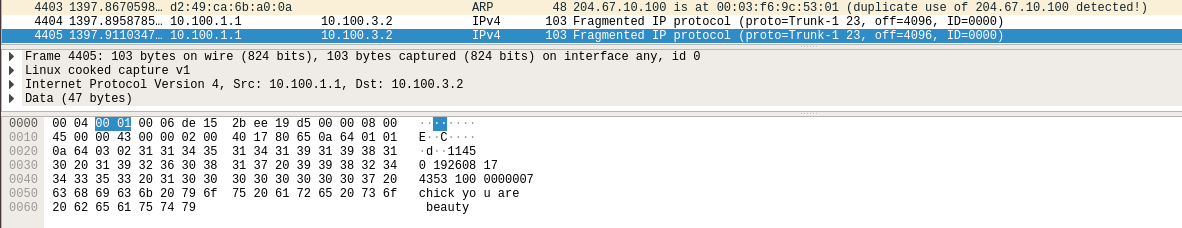
\includegraphics[width=0.9\linewidth]{../lab-netstack-premium-master/checkpoints/CP3.png}
	\caption{CP-3: The frame we send on device \texttt{ns2}}
	\label{fig:CP1}
	\end{figure}
	
	\par The IP Header locates in bit \texttt{0x0010 $\sim$ 0x0023}. and the meaning is shown in the following table.
	
	\begin{itemize}
		\item the higher 4 bits of \texttt{0x0010}: the version of IP protocol, $4$ because we use \texttt{IPv4}.
		
		\item the lower 4 bits of \texttt{0x0010}: the length of IP Header, $5$ because we use $5 \times 4 = 20$ bytes.
		
		\item \texttt{0x0011}: the type of service, we done need to set up this one, so it is filled $0$.
		
		\item \texttt{0x0012 $\sim$ 0x0013}: the length of the information, \texttt{0x43} because exactly $81$ bytes follows the header.
		
		\item \texttt{0x0014 $\sim$ 0x0015}: the identification of the packet, because the information may be fragmented. We done need to set up this one, so it is filled $0$.
		
		\item the higher $3$ bits of \texttt{0x0016}: the identification of the fragment, We done need to set up this one.
		
		\item the lower $13$ bits of \texttt{0x0016 $\sim$ 0x0017}: the offset of the fragment, used while the information is fragmented. We done need to set up this one.
		
		\item \texttt{0x0018}: the time it will survive in the server, we done need to set up this one, so it is filled \texttt{0x17} like in \texttt{pcap.trace}).
		
		\item \texttt{0x0019}: the protocol used, we done need to set up this one, so it is filled \texttt{0x17}.
		
		\item \texttt{0x001a $\sim$ 0x001b}: the checksum of packet, calculated after other terms are filled.
		
		\item \texttt{0x001c $\sim$ 0x001f}: the IP address of source, $\texttt{10.100.1.1}$ in the network.
		
		\item \texttt{0x0020 $\sim$ 0x0023}: the IP address of destination, $\texttt{10.100.3.2}$ in the network.
		
	\end{itemize}
	
	\subsection*{CP4}
	
	\par Set UP the virtual network saved in \texttt{network1.txt}. and then launch 4 bashs, each runs the server using the command
	
	\begin{lstlisting}
	sudo ./src/lab1 2 name
	\end{lstlisting}
	
	\par where name represents the name of the server locate in, like \texttt{ns1}.
	
	\par First, launch the $4$ servers at the same time, and server \texttt{ns1} will try to send a message to \texttt{ns4} after about $30$ seconds. \texttt{ns4} receive the message and it print the raw message like follow.(\texttt{ns1} on the top left, \texttt{ns4} on the bottom right, the same arrangement is used in \texttt{CP4-2,CP4-3}).
	
	\begin{figure}[htbp]
		\centering
		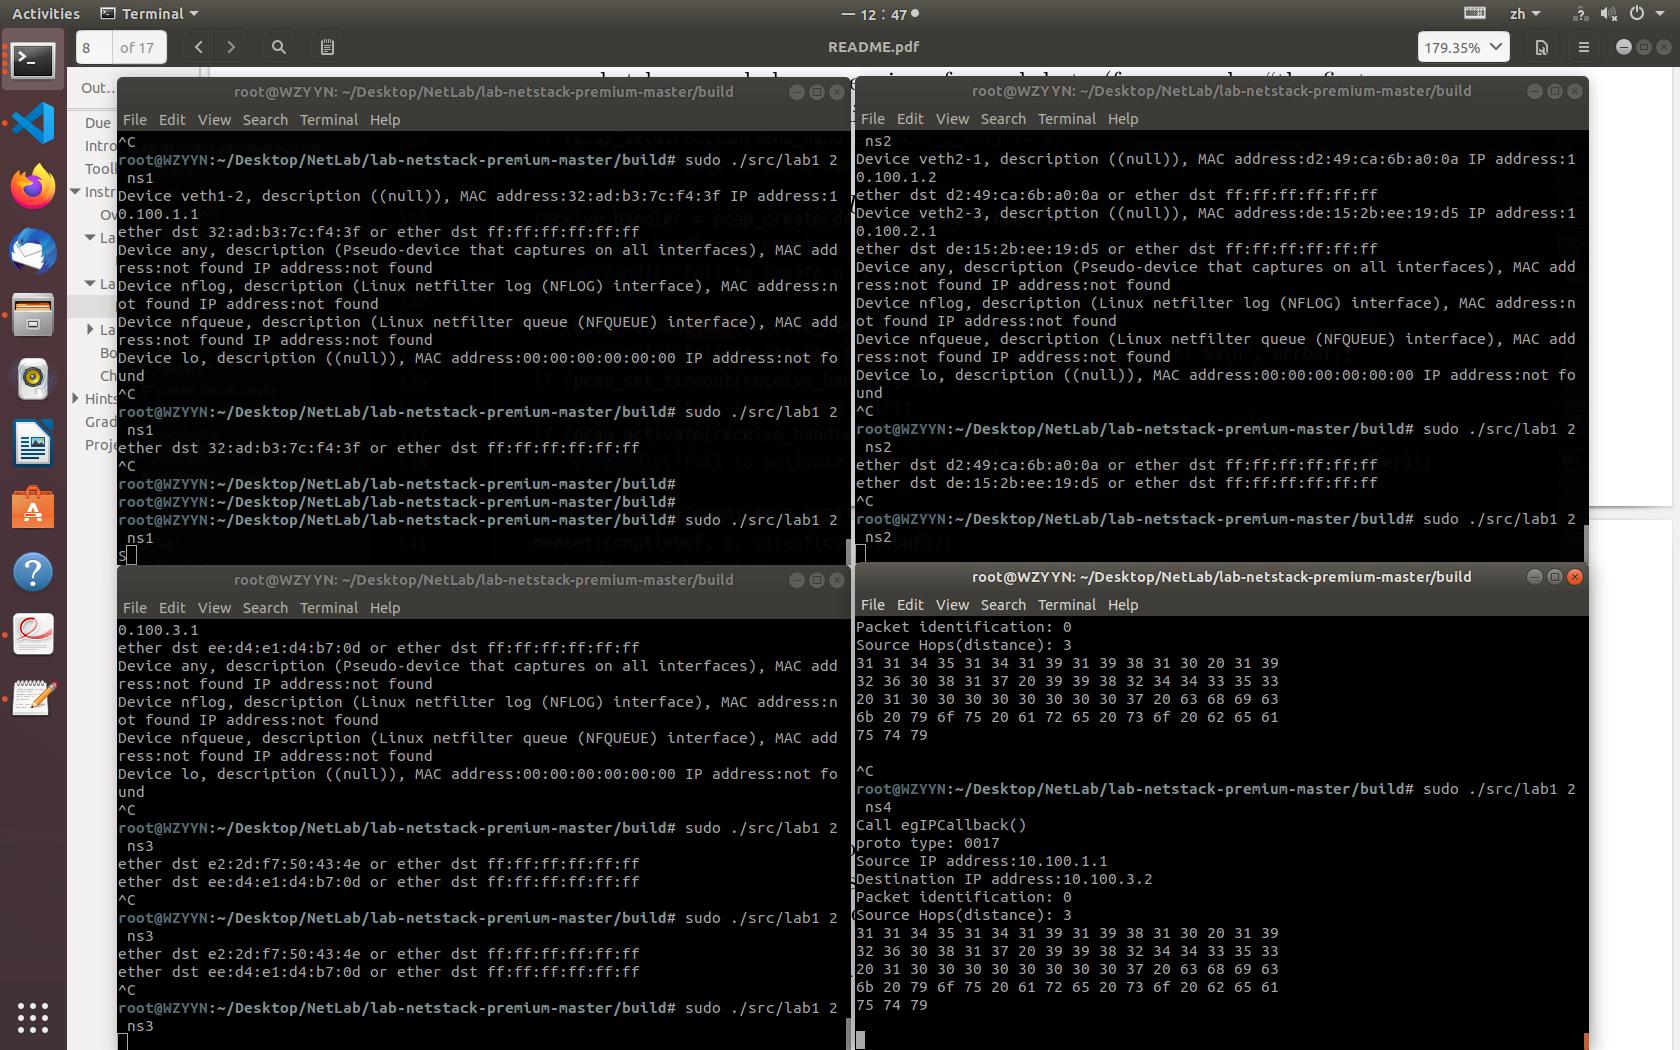
\includegraphics[width=0.9\linewidth]{../lab-netstack-premium-master/checkpoints/CP4-1.png}
		\caption{CP4-1: \texttt{ns4} receive the message from \texttt{ns1}}
		\label{fig:CP4-1}
	\end{figure}
	
	\par Then we close \texttt{ns2}, and launch \texttt{ns1} again. It will show that \texttt{ns4} is disconnected because it could not find the route to it. The image I cut is \texttt{CP4-2}.
	
	\begin{figure}[htbp]
		\centering
		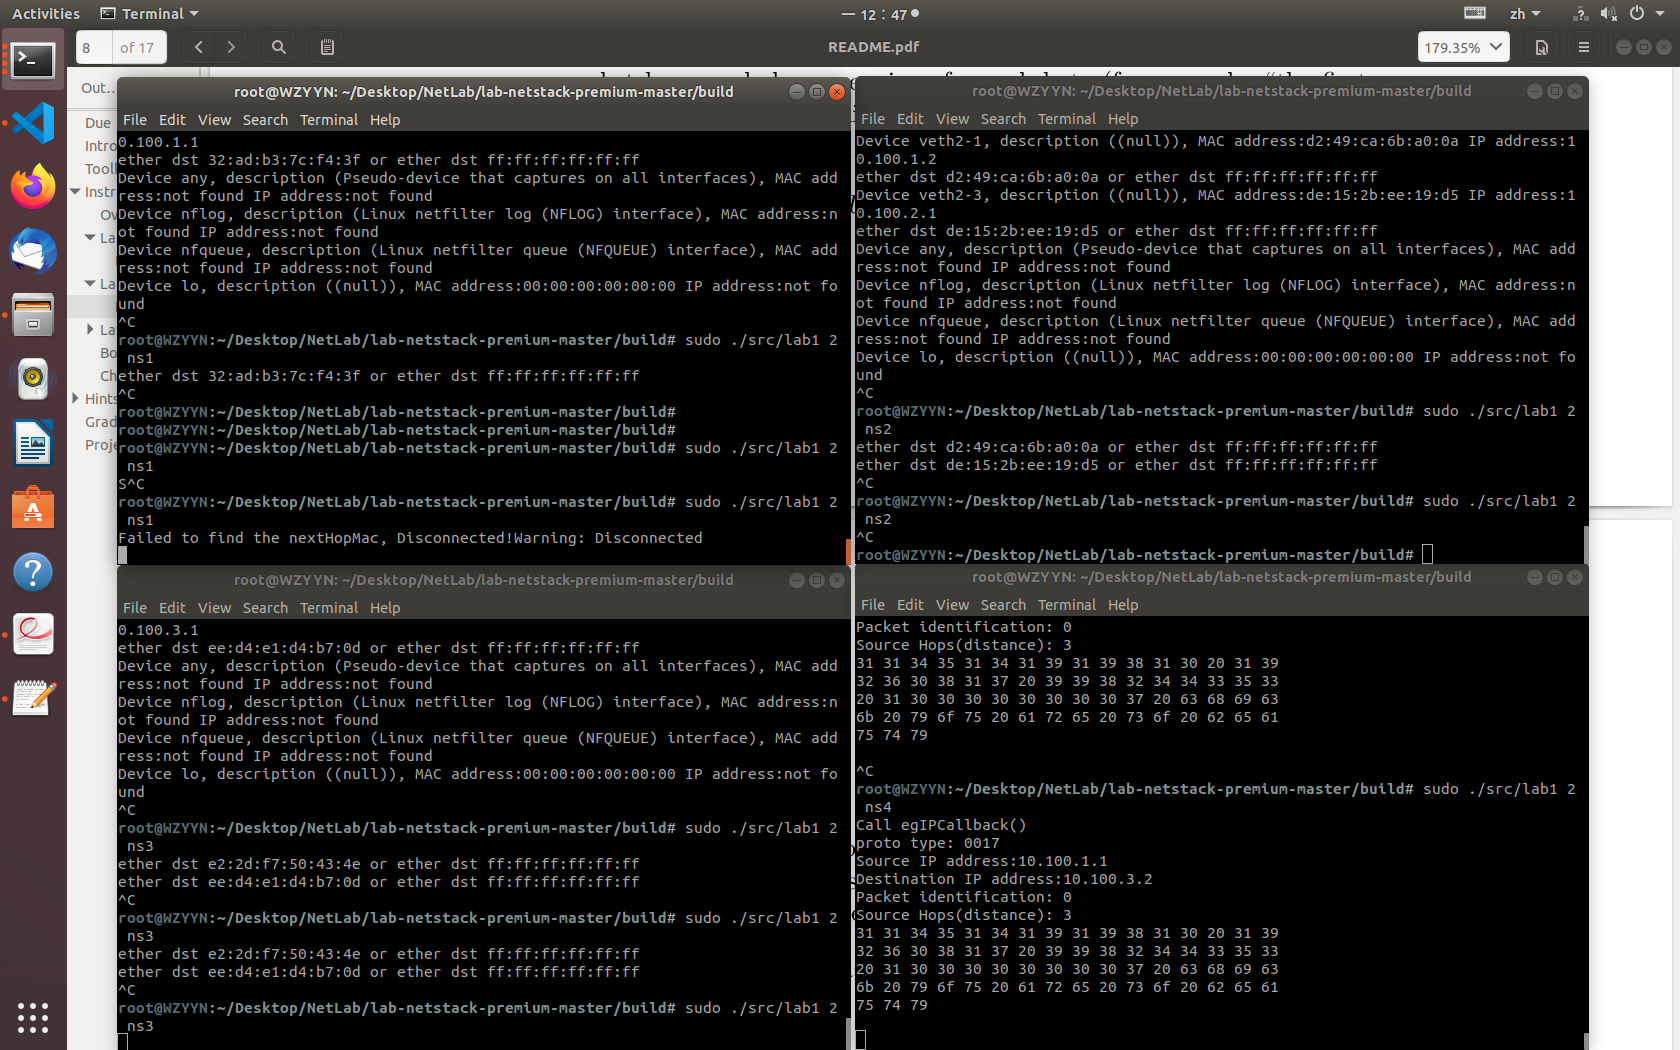
\includegraphics[width=0.9\linewidth]{../lab-netstack-premium-master/checkpoints/CP4-2.png}
		\caption{CP4-2: \texttt{ns1} shows that \texttt{ns4} is disconnected.}
		\label{fig:CP4-2}
	\end{figure}
	
	\par Finally, we launch \texttt{ns2} again. This time \texttt{ns1} could found \texttt{ns4}, and the message is successfully delivered. The image I cut is \texttt{CP4-4}.
	
	\begin{figure}[htbp]
		\centering
		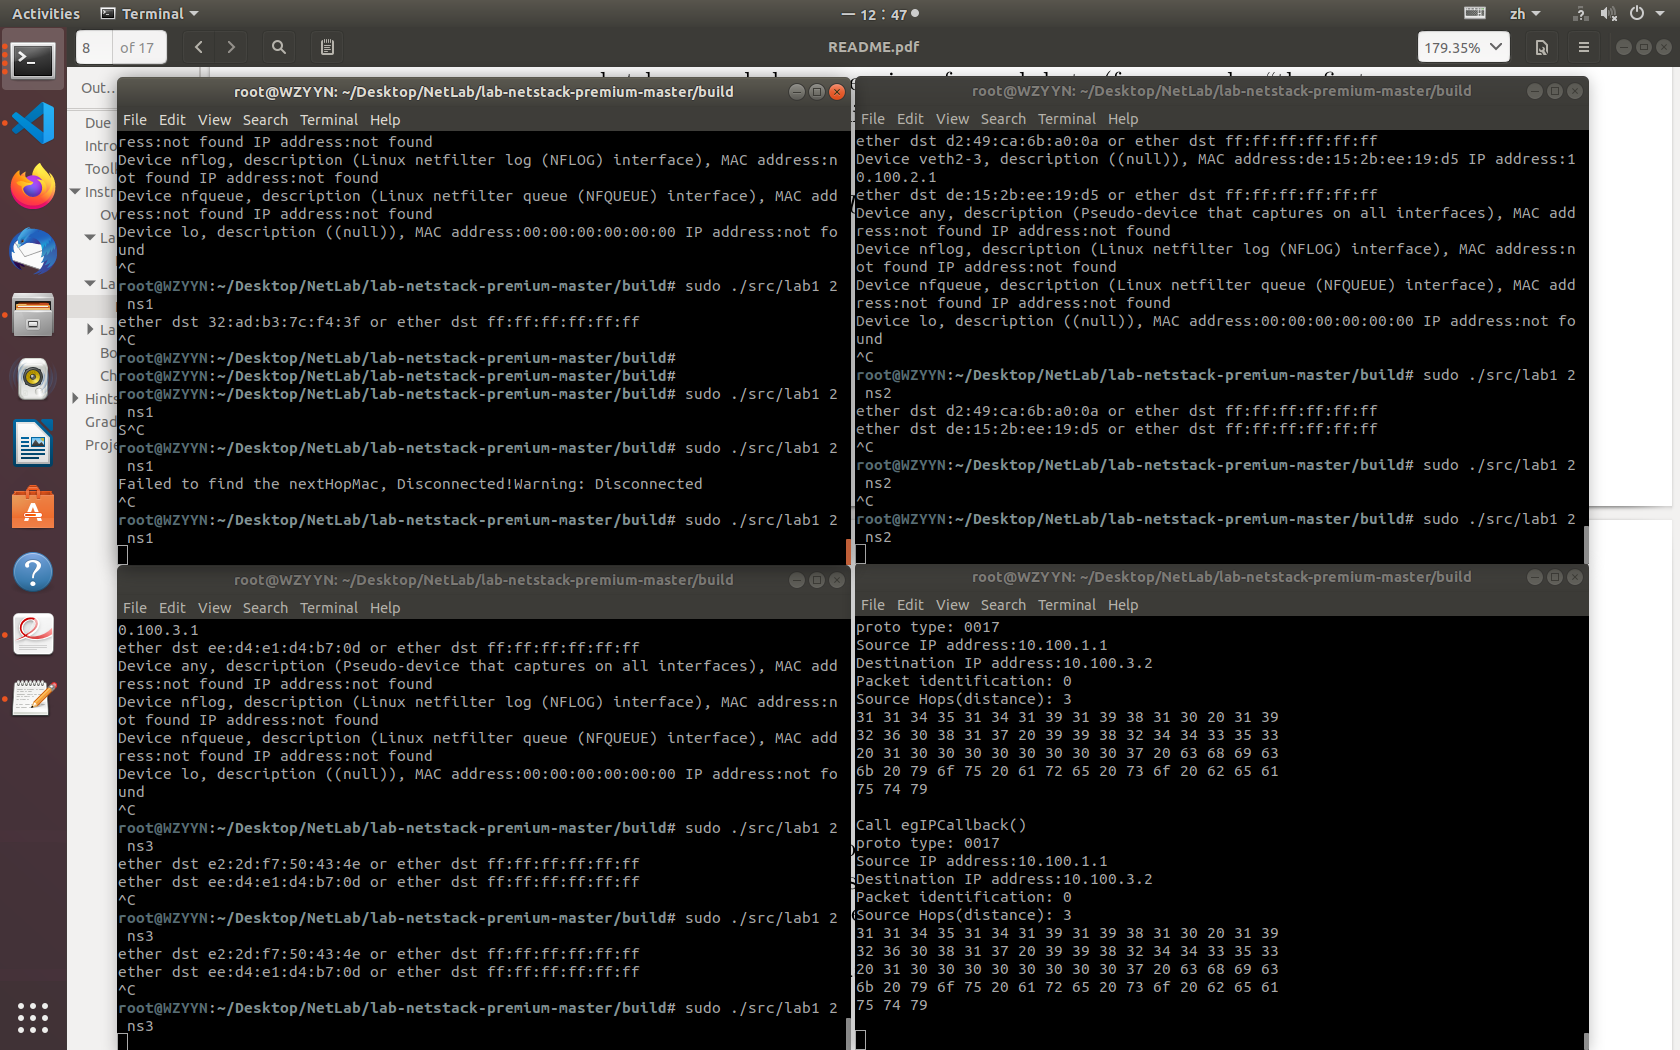
\includegraphics[width=0.8\linewidth]{../lab-netstack-premium-master/checkpoints/CP4-3.png}
		\caption{CP4-3:\texttt{ns4} receive the message from \texttt{ns1}}
		\label{fig:CP4-3}
	\end{figure}
		
	\subsection*{CP5}
	
	\par Set UP the virtual network saved in \texttt{network1.txt}. and then launch 6 bashs, each runs the server using the command
	
	\begin{lstlisting}
	sudo ./src/lab1 4 name
	\end{lstlisting}
	
		\par First, launch the $6$ servers at the same time, and each server will use my ARP-like protocol to find the distance to each other servers. If it could not found the server, the distance if set up to $-1$ represent non-exist. The output will like follow:(\texttt{ns1} on the top left, \texttt{ns6} on the bottom right, the same arrangement is used in \texttt{CP5-2}).
		
		\begin{figure}[htbp]
			\centering
			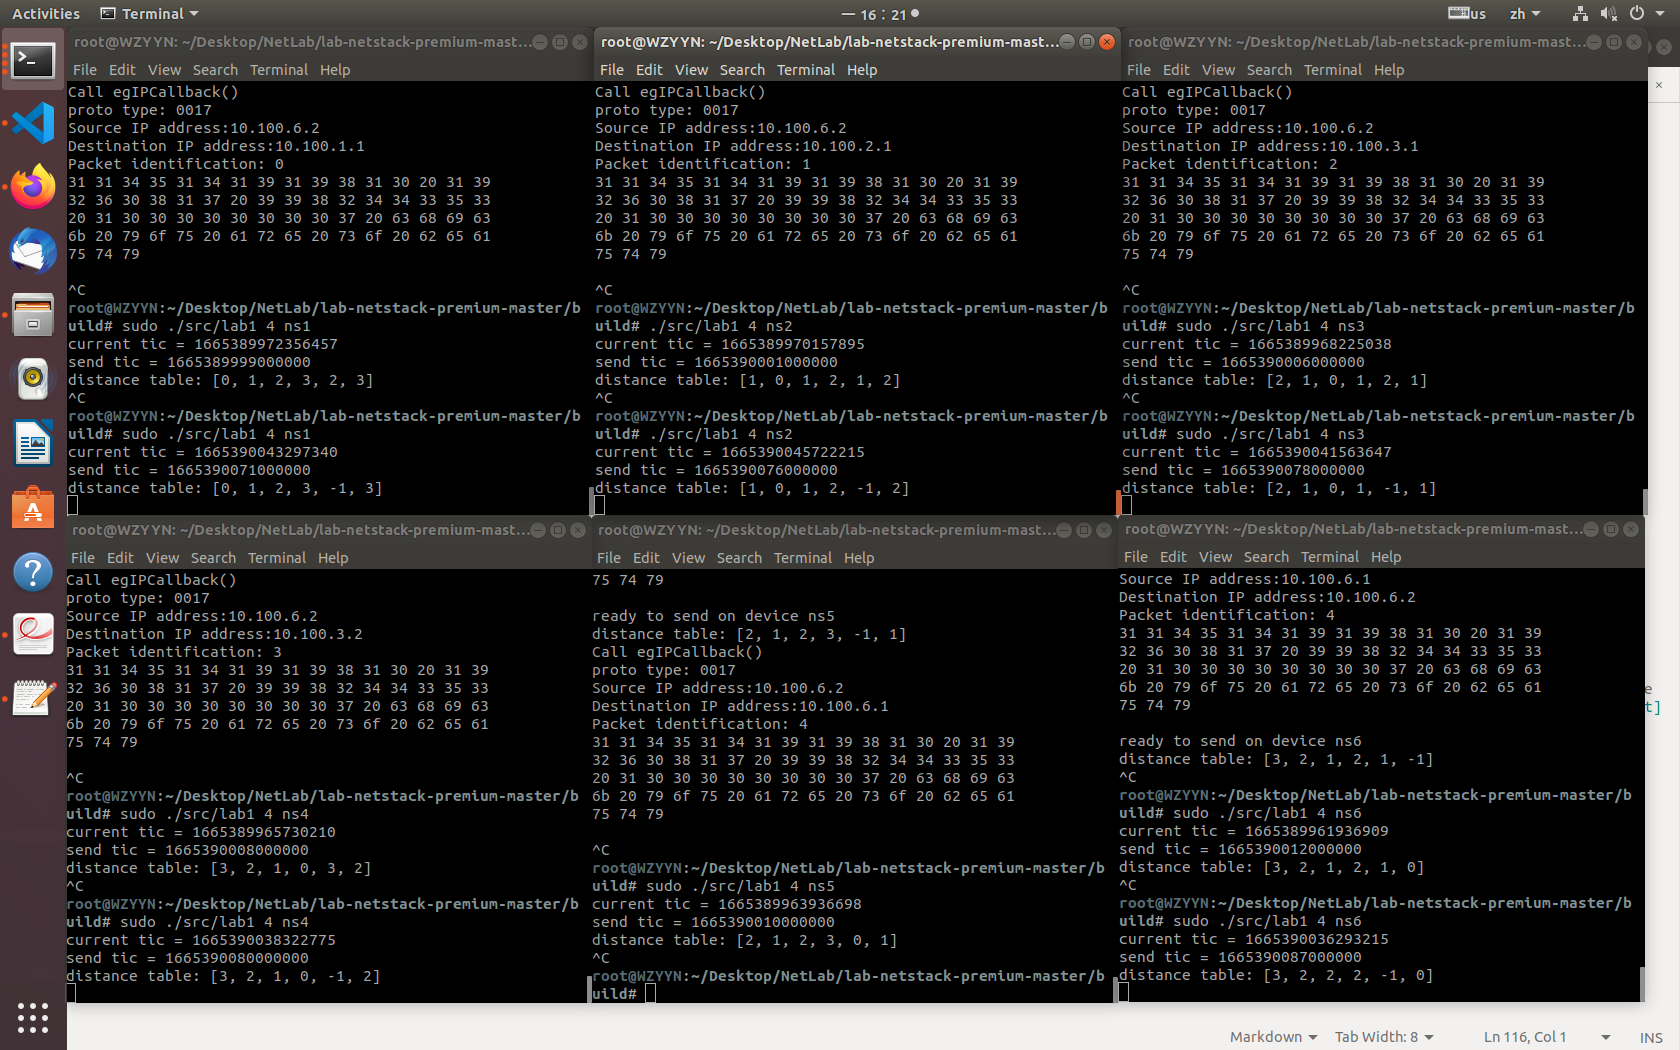
\includegraphics[width=0.9\linewidth]{../lab-netstack-premium-master/checkpoints/CP5-1.png}
			\caption{CP5-1: the distance for each pair of servers.}
			\label{fig:CP5-1}
		\end{figure}
		
		\par so the distance table look like follows:
		
		\begin{tabular}{|c|c|c|c|c|c|c|}
			\hline /&1&2&3&4&5&6\\
			\hline 1&0&1&2&3&2&3\\
			\hline 2&1&0&1&2&1&2\\
			\hline 3&2&1&0&1&2&1\\
			\hline 4&3&2&1&0&3&2\\
			\hline 5&2&1&2&3&0&1\\
			\hline 6&3&2&1&2&1&0\\
			\hline
		\end{tabular}
		
		\par After that, we only launch \texttt{ns1 $\sim$ ns4, ns6} at the same time. then the output will look like follows:
		
		\begin{figure}[htbp]
			\centering
			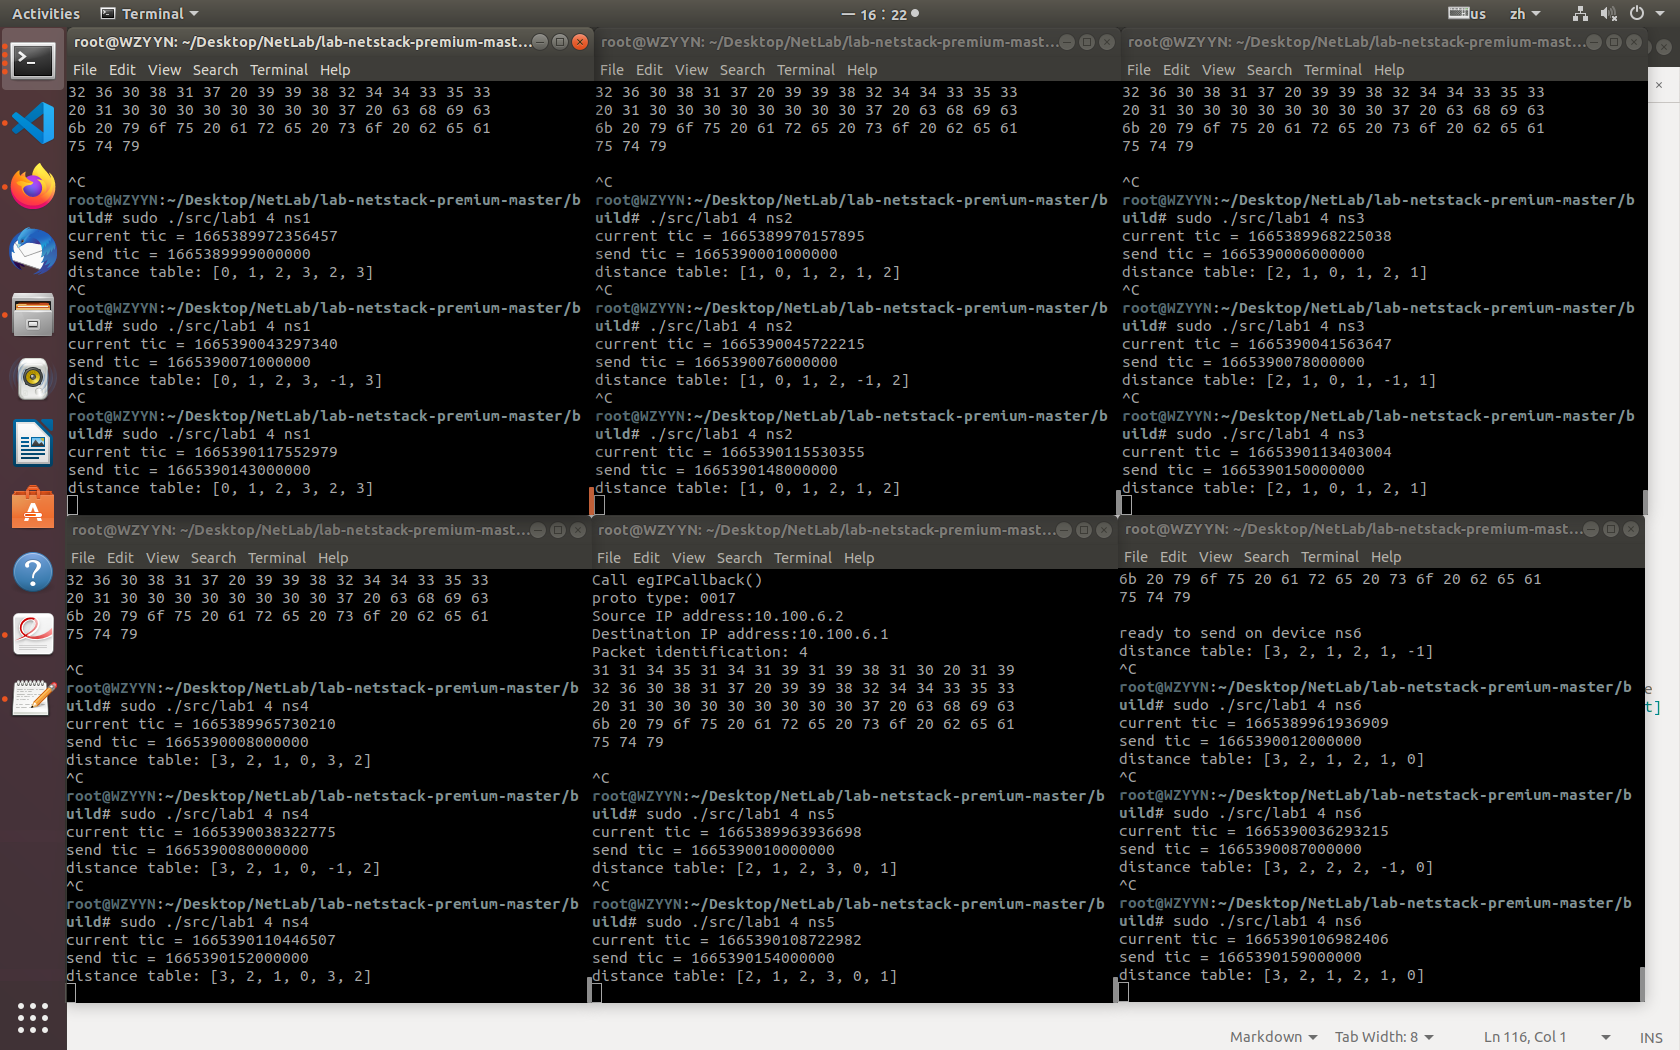
\includegraphics[width=0.9\linewidth]{../lab-netstack-premium-master/checkpoints/CP5-2.png}
			\caption{CP5-2: the distance for each pair of servers if \texttt{ns5} is not launched.}
			\label{fig:CP5-1}
		\end{figure}
		
		\par so the distance table look like follows:
		
		\begin{tabular}{|c|c|c|c|c|c|c|}
			\hline /&1&2&3&4&5&6\\
			\hline 1&0&1&2&3&-1&3\\
			\hline 2&1&0&1&2&-1&2\\
			\hline 3&2&1&0&1&-1&1\\
			\hline 4&3&2&1&0&-1&2\\
			\hline 5&-1&-1&-1&-1&-1&-1\\
			\hline 6&3&2&1&2&-1&0\\
			\hline
		\end{tabular}
	
	\subsection*{CP6}
	
	\par Launch one bash, and runs the following command
	
	\begin{lstlisting}
	sudo ./src/lab1 3 ns1
	\end{lstlisting}
	
	\par the server will try to set up 2 routing rules, where the one have mask length 16, the other have 24.
	
	\par In the first query, only the first rule fit, so the router return the macaddress of the first rule; however, the second query fit both rule, so the router returns the second rule, because it have a longer fitting length.
	
	\par the picture is shown below. 
	
	\begin{figure}[htbp]
		\centering
		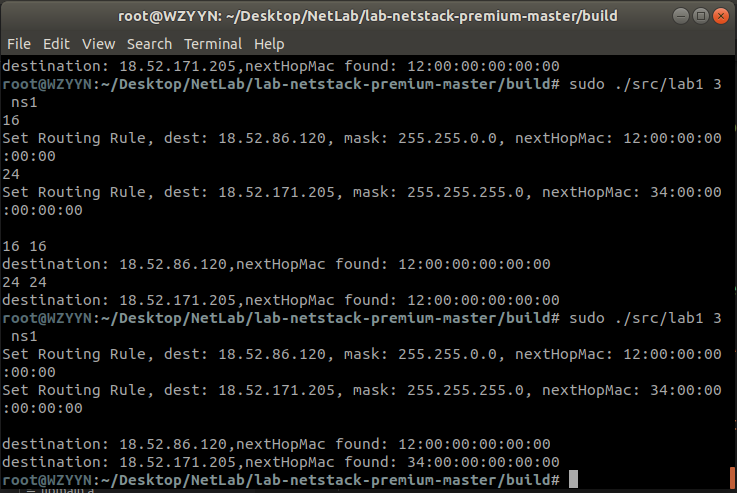
\includegraphics[width=0.9\linewidth]{../lab-netstack-premium-master/checkpoints/CP6.png}
		\caption{CP6: Example router reply.}
		\label{fig:CP5-1}
	\end{figure}
		
\end{document}